\documentclass{article}


%preamble
%required
%\usepackage{Sweave} %Integrates R code with LaTeX for creating dynamic reports
\usepackage{natbib}%Provides citation and bibliography support
\usepackage{amsmath}%Enhances mathematical typesetting capabilities.
\usepackage{textcomp}%among other things, it allows degrees C to be added
\usepackage{float}%Helps with precise figure placement using the [H] option.
\usepackage[utf8]{inputenc} % allow funny letters in citations 
\usepackage[nottoc]{tocbibind} %should add Re fences to the table of contents?
\usepackage{amsmath} % making nice equations 
\usepackage{listings} % add in stan code
\usepackage{xcolor}
\usepackage{capt-of}%allows me to set a caption for code in appendix 
\usepackage[export]{adjustbox} % adding a box around a map
\usepackage{lineno}
\linenumbers

% recommended! Uncomment the below line and change the path for your computer!
% \SweaveOpts{prefix.string=/Users/Lizzie/Documents/git/teaching/demoSweave/Fig.s/demoFig, eps=FALSE} 
%put your Fig.s in one place! Also, note that here 'Fig.s' is the folder and 'demoFig' is what each 
% Fig. produced will be titled plus its number or label (e.g., demoFig-nqpbetter.pdf')
% make your captioning look better
\usepackage[small]{caption}

\usepackage{xr-hyper} %refer to Fig.s in another document
\usepackage{hyperref}

\setlength{\captionmargin}{30pt}
\setlength{\abovecaptionskip}{0pt}
\setlength{\belowcaptionskip}{10pt}

% optional: muck with spacing
\topmargin -1.5cm        
\oddsidemargin 0.5cm   
\evensidemargin 0.5cm  % same as odd side margin but for left-hand pages
\textwidth 15.59cm
\textheight 21.94cm 
% \renewcommand{\baselinestretch}{1.5} % 1.5 lines between lines
\parindent 0pt		  % sets leading space for paragraphs
% optional: cute, fancy headers
\usepackage{fancyhdr}
\pagestyle{fancy}
%\fancyhead[LO]{Frederik Baumgarten}
%\fancyhead[RO]{Research Proposal}
% more optionals! %

\usepackage{graphicx}
\graphicspath{{/Users/frederik/github/PlantDeterminism/figures/}} % specify the path to your figures directory




\begin{document}
	
	
	% Format for a letter in "Ecology Letters"
	\title{Invest now, get paid later? Growth strategies to cope with environmental stress and benefit from extended growing seasons in a future climate %(my favourite)
		
		%dlDec18: Alternate title ideas:
		%Growth determinism/determinacy/habits in plants/woody perennials/trees: Limits and opportunities of species to time growth activities in a future climate. 
		
		%Growth determinacy in temperate trees: investing at the right time to cope with environmental stress and benefit from extended growing seasons in a future climate.
	} 
	
	\date{\today}
	\author{Frederik Baumgarten\textsuperscript{1,2}, Yann Vitasse\textsuperscript{2}, Sally?, Rob?, EM Wolkovich\textsuperscript{1}}
	\maketitle
	
	$^1$ Department of Forest and Conservation, Faculty of Forestry, University of British Columbia, 2424 Main Mall
	Vancouver, BC Canada V6T 1Z4. \\
	
	
	
	$^2$  Swiss Federal Institute for Forest, Snow and Landscape Research WSL, Zürcherstr. 111, Birmensdorf 8903, Switzerland\\ \\
	
	Corresponding Author: Frederik Baumgarten; frederik.baumgarten@ubc.ca \\
	
	%Full word count: \\
	%Summary word count: \\
	%Introduction word count: \\
	%Materials and Methods word count: \\
	%Results and figure legends word count: \\
	%Discussion word count: \\
	
	%werwolve: how is tree growth impacted by climate change? 1) by extreme events and 2) by an extended growing season? 
	%baby: better predictions of when environmental factors are influencing growth taking into account the phenological sequence of a species
	%silverbullet: concept of determinism
	
	
	

	
\section*{Abstract} %150 words
		With increasing latitude, plants are confined to a shrinking ‘time window of opportunity’ set by low temperatures (frost) and water restrictions (drought). In trees, the question of when and how much growth occurs within this window, received recently considerable attention. Thanks to high temporal resolution data of dendrometers we know that cambial cell division and differentiation occurs only within a fraction of days of the potential climatic growing season and mainly at night when cell turgor is sufficiently high. These studies contributed a lot to identify the environmental drivers and their thresholds that control growth. \\
		Yet, environmental conditions do not solely explain if a plant during the active season is growing or not. An often-overlooked factor is the phenological sequence – the developmental stages and transitions set by the genetic programming of a plant that manifests in species-specific growth patterns/habits. This internal schedule has the power to impose switches in physiological activity e.g. from structural vegetative growth to reproduction (such as fruit ripening), storage accumulation and inducing senescence despite growth-promoting conditions.\\
		Here, we revise the old concept of (in-)determinism: the ability of trees to preform tissue as an investment for next year’s growth that will overwinter in buds vs. a strategy that additionally relies on the continuous activity of the apical meristem throughout the growing season (neo formed tissue). We propose that 1) determinate species may be more resistant and resilient to environmental stressors (e.g. drought) and 2) the higher the degree of indeterminacy in a species, the greater its capacity/potential to profit from extended growing seasons. Consequently, the question of how much carbon will be sequestered in a future climate might depend not only on abiotic factors like water availability, temperature extremes and the length of the growing season, but also on the degree of determinacy set by a species' intrinsic genetic programming.\\
		
			\textbf{Keywords}: plant growth, tree phenology, shoot extension, indeterminate growers, carbon sequestration, growing season length, drought, genetic programming, phenotypic plasticity
			\newpage
	
\section*{Introduction}
	
	\subsection*{Investment by trees}
		Investing at the right time is of crucial importance for the survival and fitness of plants. While in tropical ecosystems a continued production of tissue can be both possible and advantageous, in most other regions strategies that rely on growth from stored reserves and pre-build tissue are widely common. 

	\subsection*{Introduce seasonality}
		The further one travels from the equator towards the poles, the tighter plants are confined to a shrinking ‘time window of opportunity’ set by low temperatures. Below 5°C  metabolic activity slows down to an extend where growth and development comes to a halt. More importantly, freezing temperatures can cause severe damages to plant tissue if exposed at the wrong time of development, e.g. after leaf unfolding or prior to fruit maturation. While annual plant species accommodate their entire life cycle within this window, seasonal climates urge perennials to split their growing phase into annual chunks with periods of activity alternating with a period of rest (dormancy). This is referred to as intermittent or rhythmic (as opposed to continuous) growth. \\
		
		During the active growing season also high temperatures can reduce plant activity and development, ultimately to the point where meristems fail to produce new cells and protein degradation damage the photosynthesis apparatus if species-specific thresholds are exceeded (REF). Along with higher temperatures, the vapour pressure deficit rises, which in turn drives the evaporative demand of plants. High evaporation and limited soil water availablilty, decrease the water potential in the soil and along the entire root-to-shoot-continuum. Since mitosis and differentiation requires sufficient turgor (cell pressure), decreasing water status of plants in such a drought scenario limits any further meristematic activity. Figure \ref{fig:fig_1xxx} shows these temperature and soil moisture limitations as "environmental filters". \\
		
		Given our developed physiological understanding on how growth is controlled by environmental factors, namely temperature and soil water availability, one could think that predictions about when and how much trees are growing in a current and future climate should be fairly simple to make. However, this is not the case (REF), although many studies currently tackle this research field and estimate the potential of carbon sequestration. It seems that environmental variables alone are not sufficient to capture the dynamic and extend of biomass production/carbon sequestration.  Here we propose the framework for an additional factor to consider: internal growth control - the genetically fixed developmental program that can dictate not to grow despite of favourable environmental conditions.\\
		
		While plants have evolved many mechanism to tolerate or avoid such potentially harmful conditions by specialized morphological adaptations, most species, even in the tropics cope with fluctuating temperature and moisture regimes by temporally escaping these conditions. This involves the progression of a dormancy cycle and the timing and prioritization of life history events (phenology). Plants outside the agricultural context rarely maximize biomass production (KörnerXXX). Rather they are selected for survival to increase their fitness which is tightly linked to their intrinsic programming (or phenological sequence) which imposes abrupt switches in resource allocation from vegetative growth to reproduction (flowering, fruit maturation) and storage (REF). Figure \ref{fig:fig_1xxx} shows these additional "internal filters" eventually narrowing down the window in which growth can effectively occur.

								\begin{figure}
								\centering
								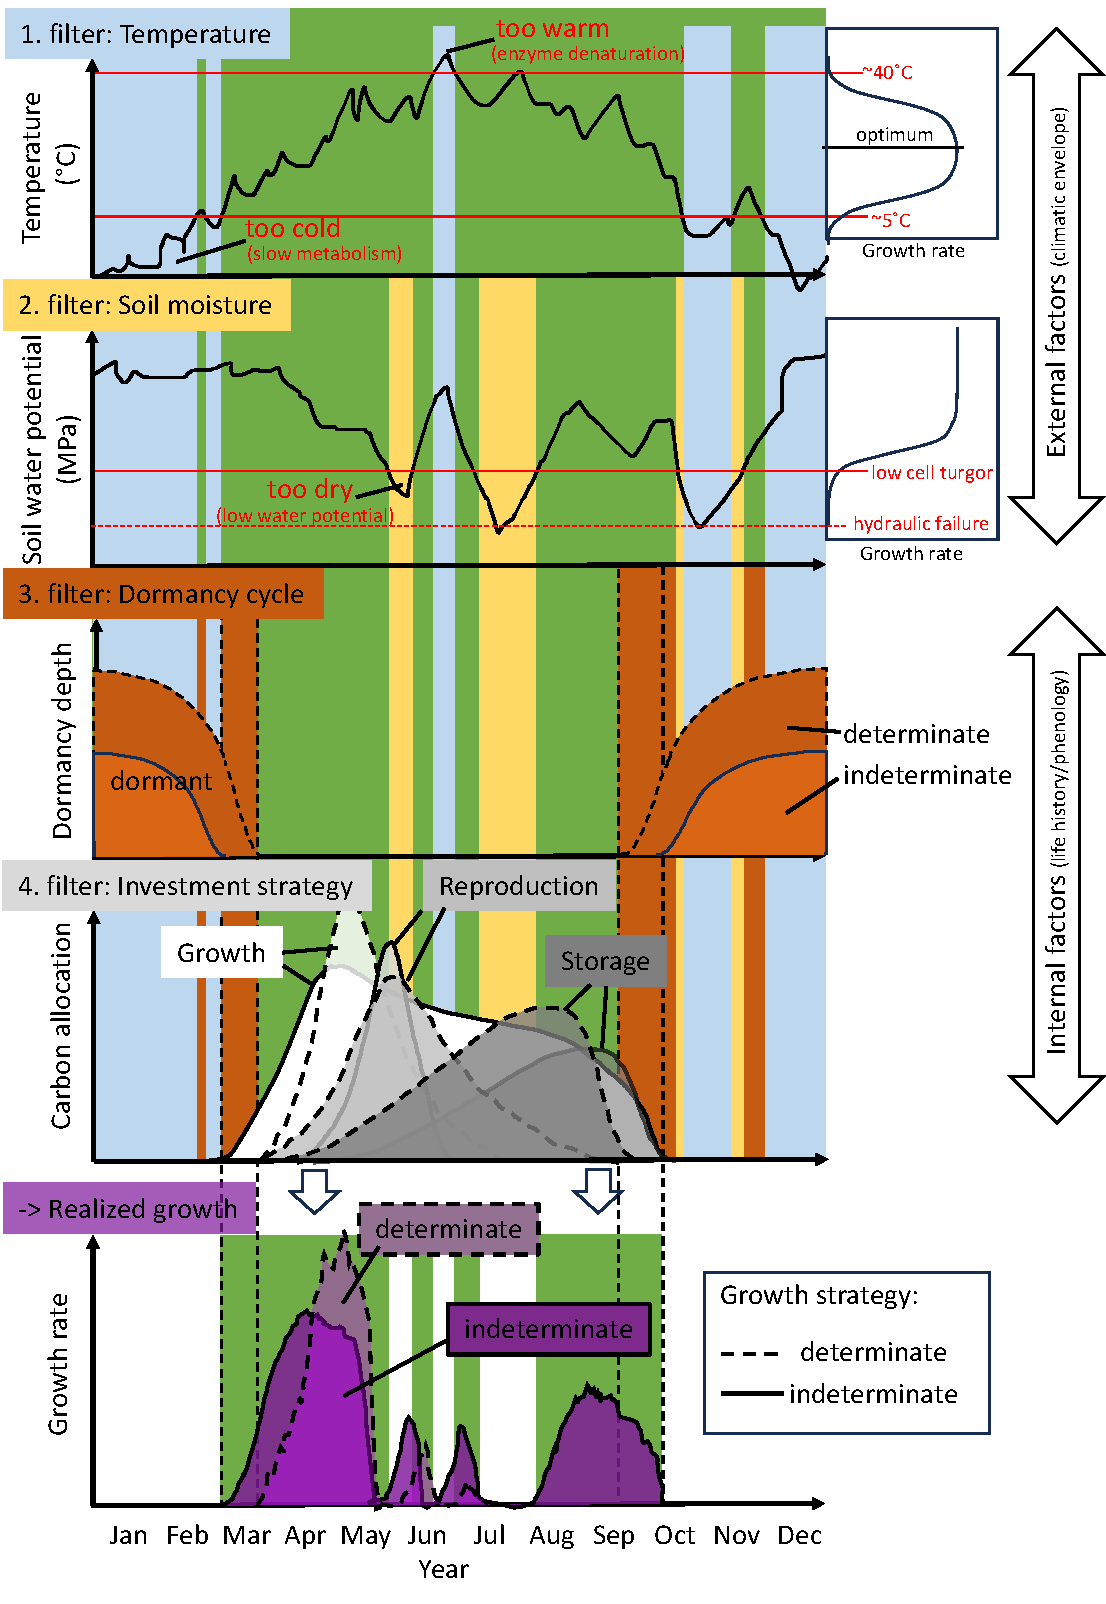
\includegraphics[width=0.9\textwidth]{Fig_1_V3.pdf} 
								\caption{Schematic overview of the discrepancy between the potential growing season and the effectively realized vegetative growth. Environmental factors like temperature and soil moisture, exceeding growth-promoting thresholds can be seen as filters that narrow the window of opportunity available for vegetative growth. The species-specific life history cycle (phenology) can further impose another filter by imposing a dormancy cycle and prioritizing developmental processes other than vegetative growth (e.g. flowering, fruit maturation and storage). }
								\label{fig:fig_1xxx}
							\end{figure}

	
\section*{The concept of (in)determinate growth}
Most of our understanding of growth strategies or habits in trees dates back to a period in the mid 1900s. Since then many different terms have entered the literature along with various definitions spanning the fields of genomics, physiology and ecology across the animal and plant kingdom. All plants add to their primary bodies as long as they live and can therefore be considered ‘indeterminate growers’ like mollusks, fish and reptiles. However, in trees the concept of determinacy refers to the ability to:\\
a) preform tissue (i.e. structural growth) as a future investment that is ready to be deployed in spring with sustained growth thereafter (determinate strategy)\\
b) maintain a somewhat constant growth activity by forming new tissue during the growing season (indeterminate strategy)\\





	history , old poplar in 70ies, many terms
	what is it? fig
	1 sentence represented as dichotomous but intermediate examples exist
	
		Figure \ref{fig:fig_2xxx} shows an example figure.
	
	 \citep{ejsmondHowTimeGrowth2010}. However, 
	
	
								\begin{figure}
								\centering
								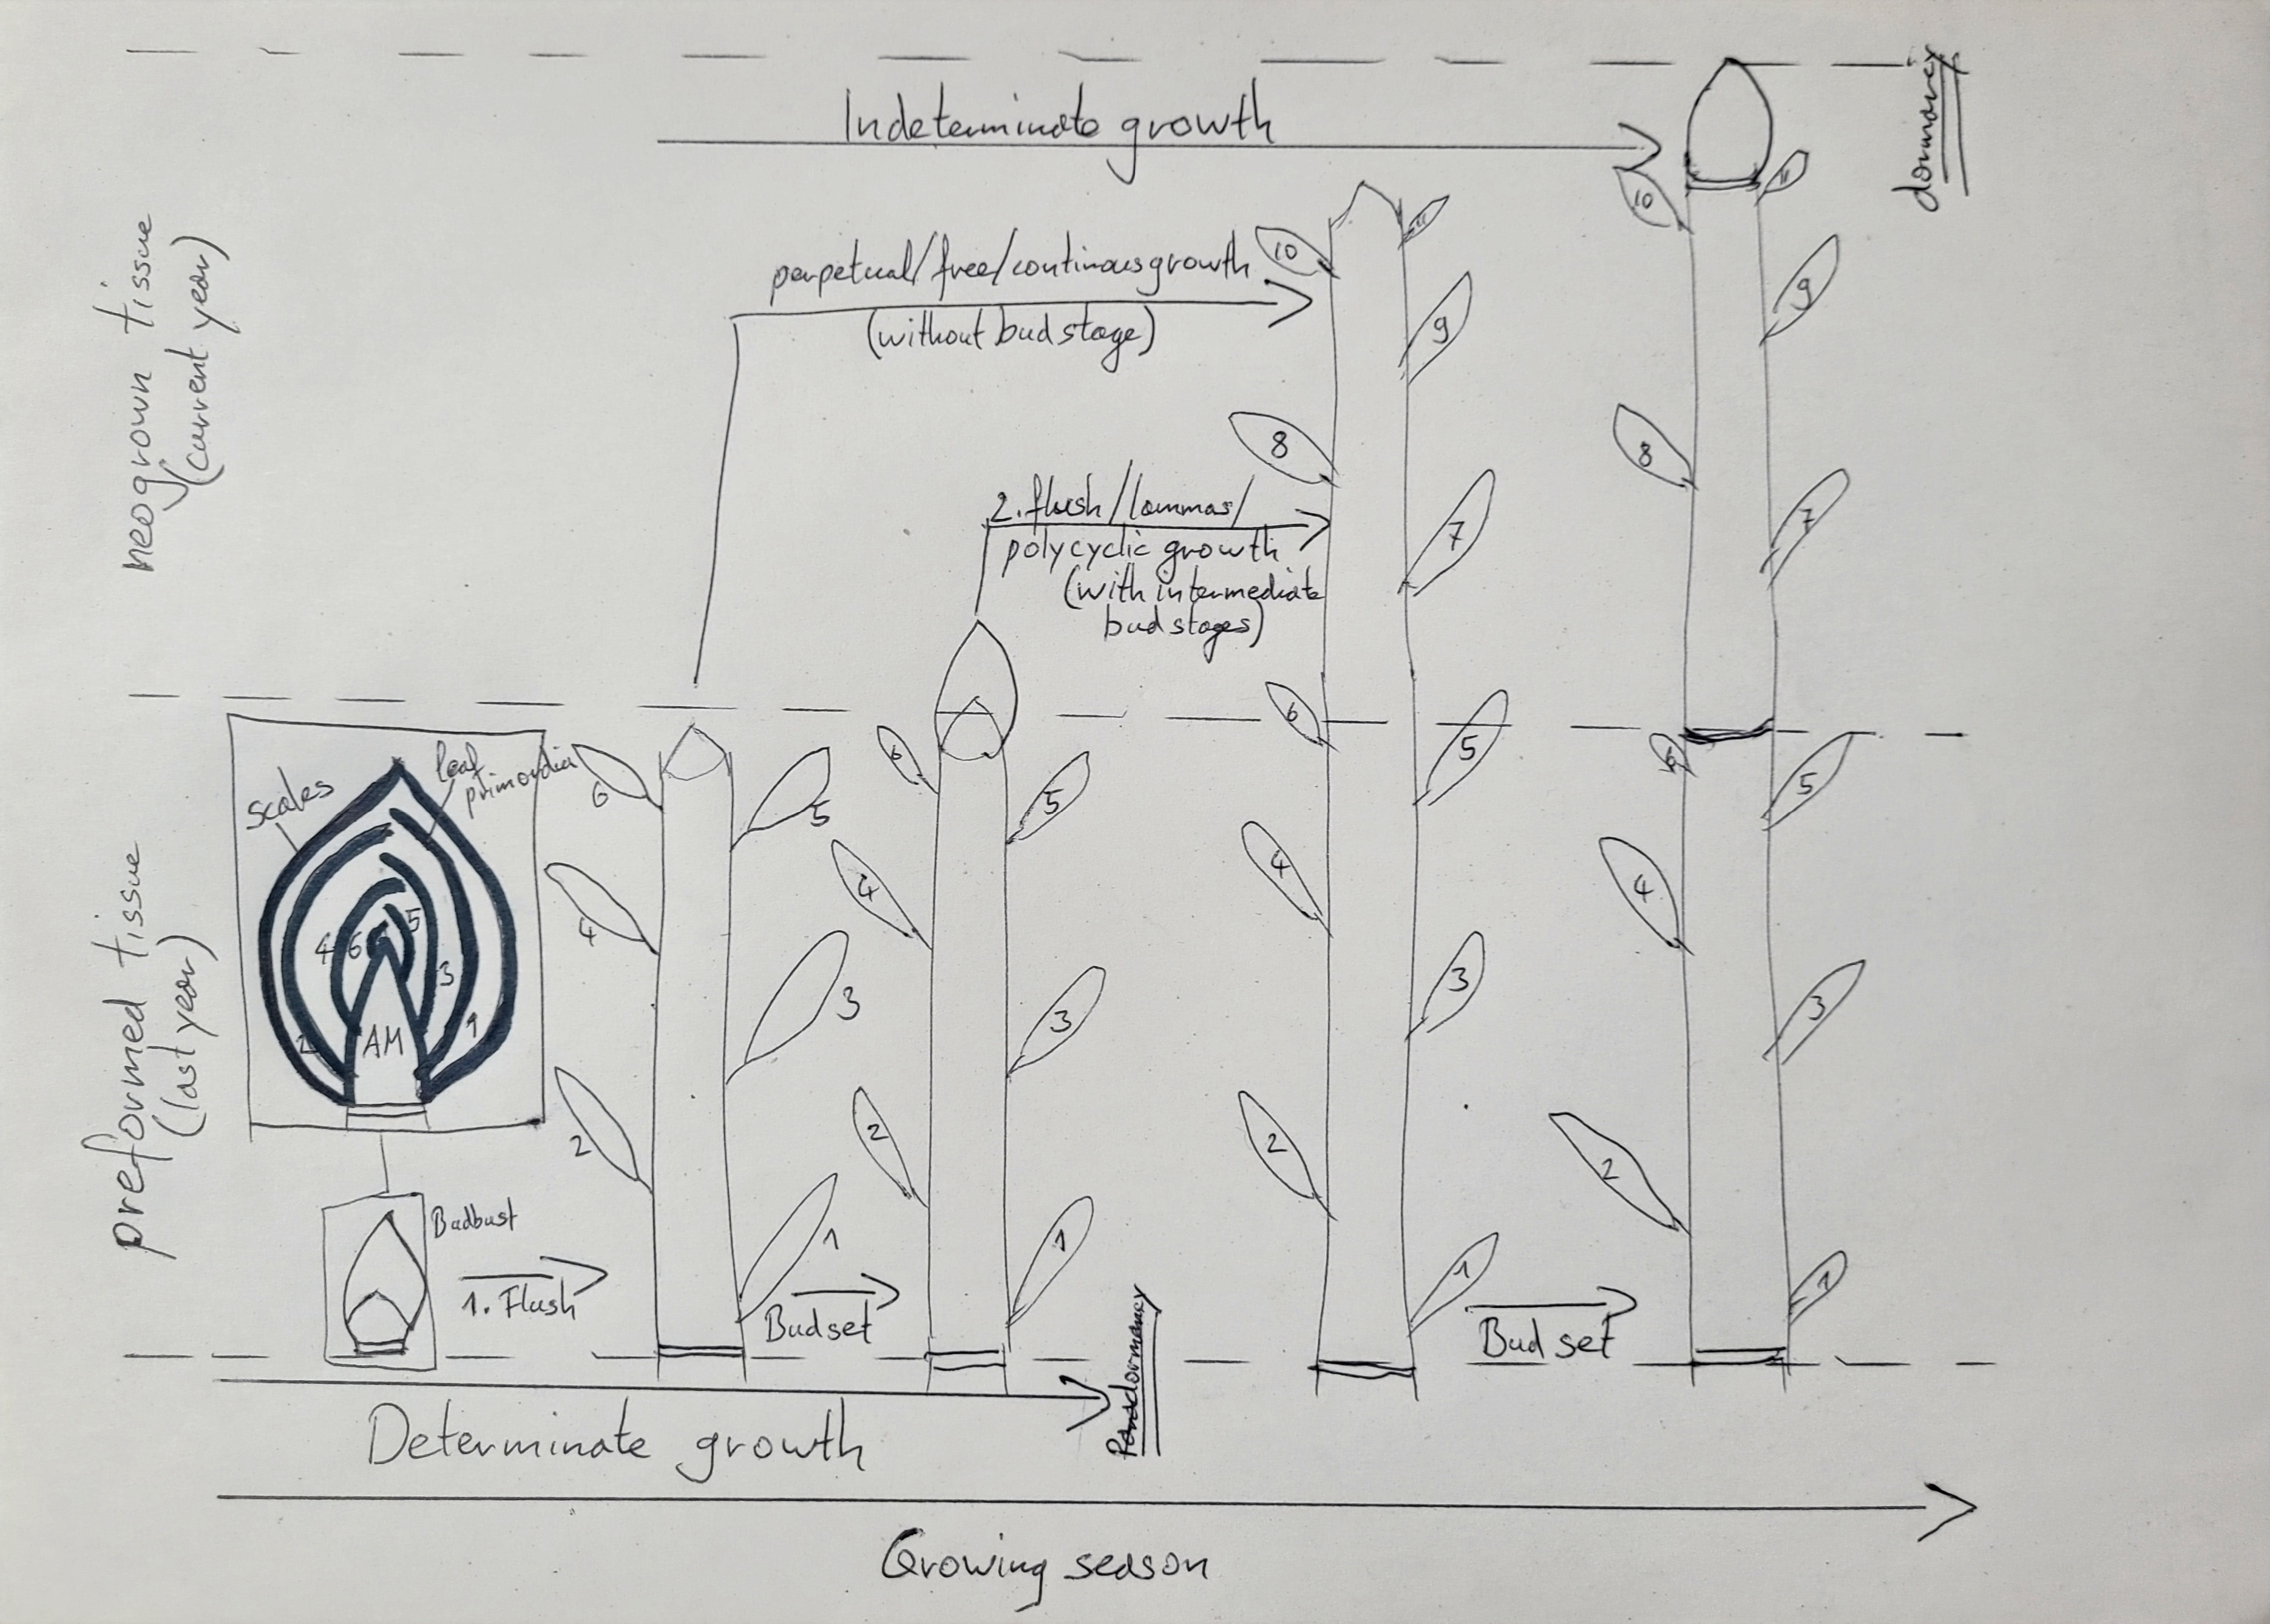
\includegraphics[width=1.1\textwidth]{Fig_2.jpg} 
								\caption{Determinate and indeterminate growth within one growing season. Commonly all tree species deploy buds during their first spring flush from prebuild and overwintering leaf primordia (A-B). Determinate growing species set bud that are under hormonal suppression (paradormancy) to sustain any further activity of the shoot apical meristem (C). Indeterminate growing species continue to produce new tissue directly (D) or through one or several intermediate bud stage(s) (E). Finally all species set their bud and enter endodormancy. Apical meristem (AM); Bud scale (BS); leaf primordia (LP).}
								\label{fig:fig_2xxx}
								\end{figure}
	
\section*{Control mechanisms/What controls/drivers of determinism}
	a)total physiology/envrironmental control 1-2 para
	warm, wet, ideal leads to indeterminate?
	but environment varies above/belowground
	R:S matters
	but this perspectives suggest you can flip species strategy completely and we do not see that.
	b) Genetically controlled /species variation see box/table/fig with list of species
	general overview of species vary
	c) these are fundamental trade-offs - both successful and co -occur in communities
	successional stage, ontogeny, life span, evolution
	
	...but will both still be successful with CC?
	
\section*{The role of determinism with climate change }
	Figure explain. temp vs. moisture vs. who wins/ phenology
	C sequestration
	
			Figure \ref{fig:fig_3xxx} shows an example figure.
	
								\begin{figure}
								\centering
								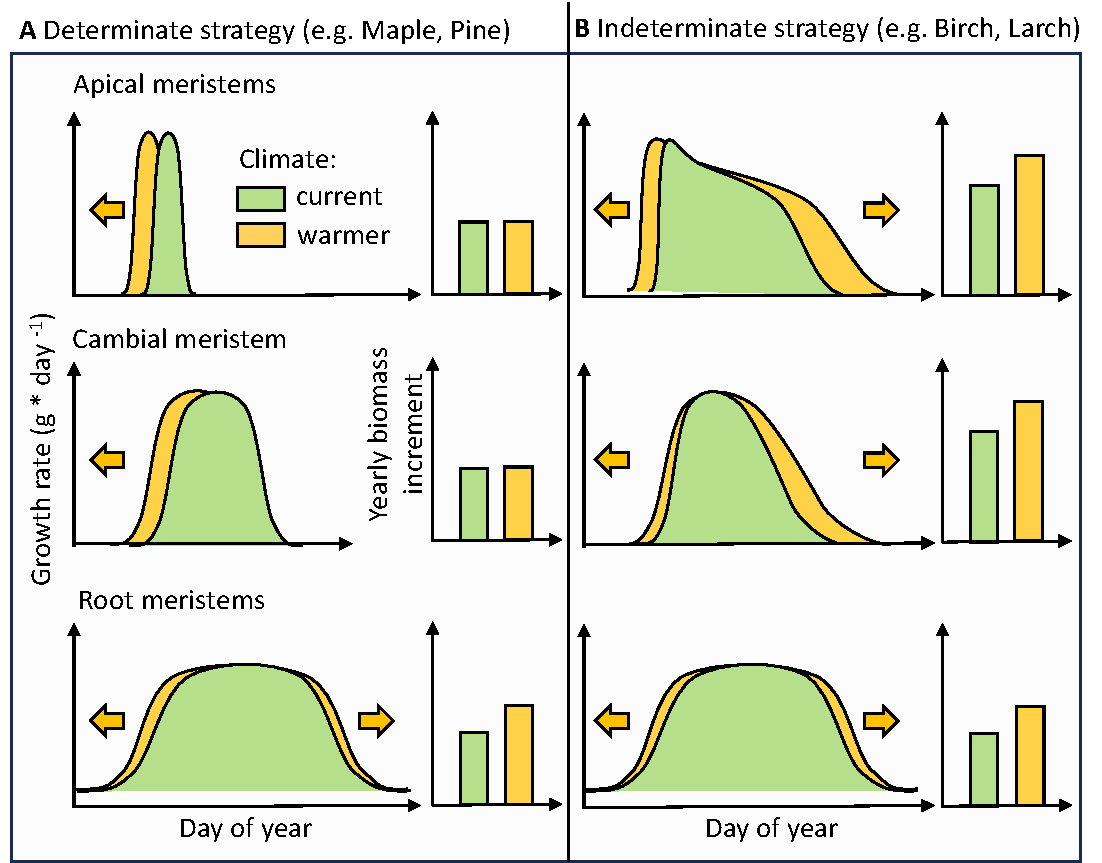
\includegraphics[width=0.9\textwidth]{Fig_3_V2.pdf} 
								\caption{Hypothesized predictions of growth rates for the three major meristems (apical, cambium and root) classes of trees under current and warmer climates following an extreme determinate (A) and indeterminate (B) growth strategy. The area under the curve is summarized as yearly biomass increment in the respective bar-plot. Arrows indicate the shift of growth phenology under warmer climate conditions. Root meristems appear to be purely temperature-opportunistic for both strategies, even growing during warm winter spells. The indicated genera were observed to showcase the illustrated trends. The responses of these two contrasting growth strategy might apply not only to different tree species but also within a population (e.g. along environmental gradients) and even within an individuum as it transitions from the junvenile to the adult stage (ontogeny).}
								\label{fig:fig_3xxx}
							\end{figure}
	
\section*{Future directions}
	Questions critical forcasting now to larger evolution questions
	
	a) (1-2 paragraphfs) how much does dezerminism predict bufferin vs. exploitation of env. change?
	explain this in simple words
	experiment phaenoflex
	
	b) How flexible are spp. in determinism?
	need an answer to get anywhere but must approach from several fields
	
	bi) Physiology: universal across meristmes? linked to xylogenesis?
	universal across allocation? (reproduction, storage and growth?)
	gene/hormones (1-2 para)
	bii) Evol. history (end on metric fortshadowing)
	
	c) better metricx
	opening....its treated dichotomy by 1 field, flexible by a different so clearly it has variability we need to understand to move forward
	
	we propose several metrics from best to worse, dificult to easy.
	(1) nleaves  EOS /n leaves in buds SOS
	
	(2) shoot elongation/dendrometers radial growth? 
	
	(3) "second flushes" in large databases? US national forest network 
	NDVI second flushes?
	
	


	
	

	
	\pagebreak
	

	

	

	
	\newpage
	
	\bibliography{Growth_determination}
	\bibliographystyle{ecolett}
	
	
	
\end{document}






